\begin{center}

\includegraphics[width=0.6\textwidth]{content/3/chapter4/images/36.png}\\
Cippi在欣赏钻石
\end{center}

C++20中,有了两个新的关键字:consteval和constinit。关键字consteval生成一个在编译时执行的函数,constinit保证变量在编译时初始化。现在,可能会觉得这两个说明符都与constexpr非常相似,你是对的。在比较关键字consteval、constinit、constexpr和const之前,先来介绍一下新的说明符consteval和constinit。

\subsubsubsection{4.5.1\hspace{0.2cm}consteval}

consteval会创建了一个“直接函数”。

\hspace*{\fill} \\ %插入空行
\noindent
\textbf{consteval函数}
\begin{lstlisting}[style=styleCXX]
consteval int sqr(int n) {
	return n * n;
}
\end{lstlisting}

每次调用立即函数都会创建一个编译时常数。更直接地说,consteval(立即)函数在编译时执行。

consteval不能应用于析构函数,或具有分配或释放内存的函数。在声明中最多只能使用consteval、constexpr或constinit说明符中的一种。直接函数(consteval)是隐式内联的,必须满足constexpr函数的要求。

C++14中constexpr函数,以及consteval函数的要求:

\begin{itemize}
\item 
consteval(constexpr)函数可以有
\begin{itemize}
\item 
有条件跳转指令或循环指令。

\item 
有多个指令。

\item 
调用constexpr函数。consteval函数只能调用constexpr函数,反之则不行。

\item 
必须使用基本数据类型作为常量表达式初始化的变量。
\end{itemize}

\item 
consteval (constexpr)函数不能有
\begin{itemize}
\item 
拥有静态或thread\_local数据。

\item 
try块或goto指令。

\item 
使用或使用非consteval函数。

\item 
使用或使用非constexpr数据。
\end{itemize}
\end{itemize}

简而言之:consteval函数的所有依赖项都必须在编译时可解析。

constevalSqr.cpp使用了consteval函数sqr。

\hspace*{\fill} \\ %插入空行
\noindent
\textbf{consteval函数}
\begin{lstlisting}[style=styleCXX]
// constevalSqr.cpp

#include <iostream>

consteval int sqr(int n) {
	return n * n;
}

int main() {

	std::cout << "sqr(5): " << sqr(5) << '\n';
	
	const int a = 5;
	std::cout << "sqr(a): " << sqr(a) << '\n';
	
	int b = 5;
	// std::cout << "sqr(b): " << sqr(b) << '\n'; ERROR

}
\end{lstlisting}

数字5是一个常量表达式,可以用作函数sqr的参数(第11行),变量a也是如此(第13行)。常量变量(如a)在用常量表达式初始化时,可在常量表达式中使用。变量b(第16行)不是常量表达式。因此,sqr(b)(第17行)的调用无效。

下面是程序的输出:

\begin{tcblisting}{breakable,commandshell={}}
sqr(5): 25
sqr(a): 25
\end{tcblisting}

\subsubsubsection{4.5.2\hspace{0.2cm}constinit}

constinit可以应用于具有静态或线程存储的变量。

\begin{itemize}
\item 
全局(命名空间)变量、静态变量或静态类成员具有静态存储的变量。这些对象在程序启动时分配,在程序结束时释放。

\item 
thread\_local变量具有线程存储的变量。为使用此数据的每个线程创建线程本地数据。thread\_local数据专属于线程,它们在第一次使用时创建,其生存期与所属线程的生存期绑定。线程本地数据通常称为线程本地存储变量。
\end{itemize}

constinit在编译时,可确保对这类变量(静态存储或线程存储的变量)进行初始化。不过,constinit并不意味着常量性(consteness)。

\hspace*{\fill} \\ %插入空行
\noindent
\textbf{使用constinit初始化}
\begin{lstlisting}[style=styleCXX]
// constinitSqr.cpp

#include <iostream>

consteval int sqr(int n) {
	return n * n;
}

constexpr auto res1 = sqr(5);
constinit auto res2 = sqr(5);

int main() {
	std::cout << "sqr(5): " << res1 << '\n';
	std::cout << "sqr(5): " << res2 << '\n';
	
	constinit thread_local auto res3 = sqr(5);
	std::cout << "sqr(5): " << res3 << '\n';
}
\end{lstlisting}

res1和res2是具有静态存储的变量。res3具有线程存储的变量。

\begin{tcblisting}{breakable,commandshell={}}
sqr(5): 25
sqr(5): 25
sqr(5): 25
\end{tcblisting}

是时候来了解一下const、constexpr、consteval和constinit的区别了。

首先,来讨论一下函数执行和变量的初始化。

\subsubsubsection{4.5.3\hspace{0.2cm}函数执行}

consteval.cpp有三个版本的square函数。

\begin{lstlisting}[style=styleCXX]
// consteval.cpp

#include <iostream>

int sqrRunTime(int n) {
	return n * n;
}

consteval int sqrCompileTime(int n) {
	return n * n;
}

constexpr int sqrRunOrCompileTime(int n) {
	return n * n;
}

int main() {

	// constexpr int prod1 = sqrRunTime(100); ERROR
	constexpr int prod2 = sqrCompileTime(100);
	constexpr int prod3 = sqrRunOrCompileTime(100);

	int x = 100;
	
	int prod4 = sqrRunTime(x);
	// int prod5 = sqrCompileTime(x); ERROR
	int prod6 = sqrRunOrCompileTime(x);
}
\end{lstlisting}

普通函数sqrRunTime(第5行)在运行时运行,consteval函数sqrCompileTime在编译时运行(第9行),constexpr函数sqrRunOrCompileTime可以在编译时或运行时运行。因此,在编译时使用sqrRunTime(第19行)是一个错误,因此,使用非常量表达式作为sqrCompileTime(第26行)的参数也是一个错误。

constexpr函数sqrRunOrCompileTime和consteval函数sqrCompileTime之间的区别在于,当上下文需要编译时求值时,sqrRunOrCompileTime必须在编译时执行。

\hspace*{\fill} \\ %插入空行
\noindent
\textbf{编译时和运行时执行}
\begin{lstlisting}[style=styleCXX]
static_assert(sqrRunOrCompileTime(10) == 100); // compile time
int arrayNewWithConstExpressiomFunction[sqrRunOrCompileTime(100)]; // compile time
constexpr int prod = sqrRunOrCompileTime(100); // compile time

int a = 100;
int runTime = sqrRunOrCompileTime(a); // run time

int runTimeOrCompiletime = sqrRunOrCompileTime(100); // run time or compile time

int alwaysCompileTime = sqrCompileTime(100); // compile time
\end{lstlisting}

第1-3行需要编译时计算。第6行只能在运行时求值,因为a不是常量表达式。关键线是第8行,函数可以在编译时或运行时执行,它在编译时执行还是在运行时执行,可能取决于编译器或优化级别。这一观察结果不适用于第10行,因为consteval函数总是在编译时执行。

\subsubsubsection{4.5.4\hspace{0.2cm}变量的初始化}

在constexprConstinit.cpp中比较一下const、constexpr和constinit。

\begin{lstlisting}[style=styleCXX]
// constexprConstinit.cpp

#include <iostream>

constexpr int constexprVal = 1000;
constinit int constinitVal = 1000;

int incrementMe(int val){ return ++val;}

int main() {
	
	auto val = 1000;
	const auto res = incrementMe(val);
	std::cout << "res: " << res << '\n';
	
	// std::cout << "res: " << ++res << '\n'; ERROR
	// std::cout << "++constexprVal: " << ++constexprVal << '\n'; ERROR
	std::cout << "++constinitVal: " << ++constinitVal << '\n';
	
	constexpr auto localConstexpr = 1000;
	// constinit auto localConstinit = 1000; ERROR

}
\end{lstlisting}

只有const变量(第13行)在运行时初始化,constexpr和constinit变量在编译时初始化。

constinit(第18行)并不意味着常量化,就像const(第16行)或constexpr(第17行)一样。声明了constexpr(第20行)或const(第13行)的变量可以创建为局部变量,但不能创建声明了constinit变量(第21行)。

\begin{tcblisting}{breakable,commandshell={}}
res: 1001
++constinitVal: 1001
\end{tcblisting}

\subsubsubsection{4.5.5\hspace{0.2cm}解决静态初始化顺序错误}

根据\href{https://isocpp.org/wiki/faq/ctors#static-init-order}{isocpp.org的FAQ},静态初始化顺序错误是“一种导致程序崩溃的微妙方式”。问题解答写道:“在C++中,静态初始化顺序是C++中一个非常微妙,且经常被误解的问题。”

在继续之前,我想做一个简短的免责声明。在不同的翻译单元中,对具有静态存储(短静态)的变量的依赖通常是一种\textit{代码异味},是需要重构的信号。因此,若愿意按照我的建议进行重构,可以跳过本节。

\hspace*{\fill} \\ %插入空行
\noindent
\textbf{4.5.5.1\hspace{0.2cm}静态初始化顺序失败}

翻译单元中的静态变量是根据定义顺序进行初始化的。

相反,在翻译单元之间初始化静态变量有一个严重的问题。当在一个翻译单元中定义了一个静态变量staticA,而在另一个翻译单元中定义了另一个静态变量staticB,并且staticB需要staticA来初始化自己时,这就会出现静态初始化顺序失败。程序呈现病态,因为不能保证哪个静态变量在(动态)运行时首先初始化。

介绍解决方案之前,来展示一下静态初始化顺序错误的例程。

\hspace*{\fill} \\ %插入空行
\noindent
\textbf{4.5.5.1.1\hspace{0.2cm}对与错,五五开}

静态函数的初始化有什么独特之处?静态函数的初始化顺序分为两个步骤:静态和动态。

当一个静态对象不能在编译时进行常量初始化时,它是不初始化的。在运行时,对这些不初始化的静态数据进行动态初始化。

\begin{lstlisting}[style=styleCXX]
// sourceSIOF1.cpp
int square(int n) {
	return n * n;
}
auto staticA = square(5);
\end{lstlisting}

\begin{lstlisting}[style=styleCXX]
// mainSOIF1.cpp

#include <iostream>

extern int staticA;
auto staticB = staticA;

int main() {
	
	std::cout << '\n';
	
	std::cout << "staticB: " << staticB << '\n';
	
	std::cout << '\n';

}
\end{lstlisting}

第5行声明静态变量staticA,staticB的初始化依赖于staticA的初始化。但是staticB在编译时未初始化,在运行时动态初始化。因为staticA和staticB属于不同的翻译单元,所以问题在于不能保证初始化staticA或staticB的顺序。staticB为0或25的概率各为50\%。

为了演示这个问题,我可以改变目标文件的链接顺序。这也改变了staticB的值!

\begin{center}
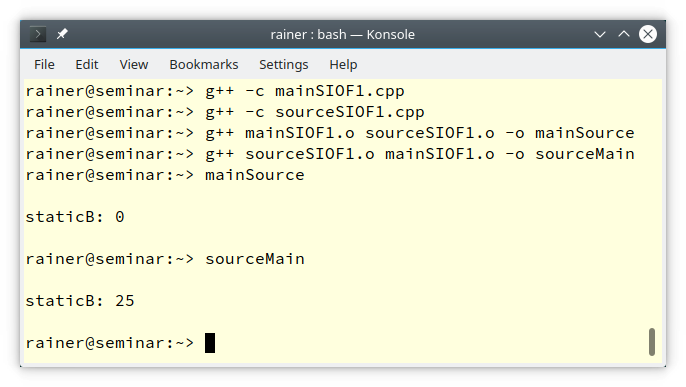
\includegraphics[width=0.8\textwidth]{content/3/chapter4/images/37.png}\\
实践静态初始化顺序错误
\end{center}

失败了吧!可执行文件的结果取决于目标文件的链接顺序。当没有C++20时,能为此做些什么呢?

\hspace*{\fill} \\ %插入空行
\noindent
\textbf{4.5.5.1.2\hspace{0.2cm}惰性初始化——局部作用域的静态对象}

局部作用域的静态变量是在首次使用时创建的。局部作用域本质上是静态变量,以某种方式被大括号包围。这种惰性创建是C++98提供的保证。在C++11中,具有局部作用域的静态变量也以线程安全的方式初始化。线程安全的\href{https://en.wikipedia.org/wiki/Scott_Meyers}{Meyers}单例就是基于这个保证。

惰性初始化也可以用来避免静态初始化顺序错误。

\begin{lstlisting}[style=styleCXX]
// sourceSIOF2.cpp

int square(int n) {
	return n * n;
}

int& staticA() {
	
	static auto staticA = square(5);
	return staticA;

}
\end{lstlisting}

\begin{lstlisting}[style=styleCXX]
// mainSOIF2.cpp

#include <iostream>

int& staticA();

auto staticB = staticA();

int main() {
	
	std::cout << '\n';
	
	std::cout << "staticB: " << staticB << '\n';
	
	std::cout << '\n';

}
\end{lstlisting}

在本例中,staticA(sourceSIOF2.cpp文件中的第9行)是局部作用域中的静态函数。mainSOIF2.cpp文件中的第5行声明了函数staticA,该函数用于在下面的行staticB中初始化。这个staticA的局部作用域保证在运行时第一次使用staticA时创建并初始化它。这种情况下,改变链接顺序不会改变staticB的值。

\begin{center}
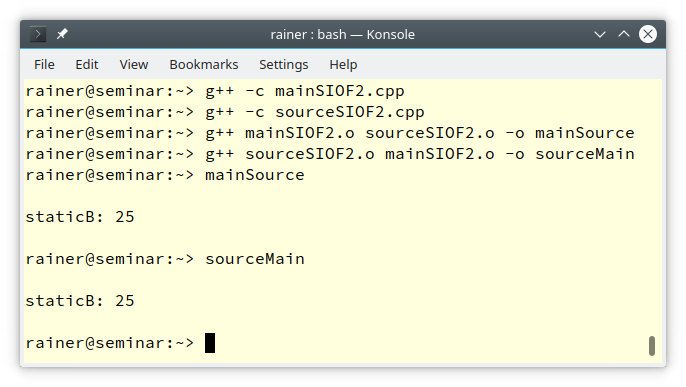
\includegraphics[width=0.6\textwidth]{content/3/chapter4/images/38.png}\\
使用本地静态变量解决静态初始化顺序问题
\end{center}

最后一步,我使用C++20解决了静态初始化顺序错误。

\hspace*{\fill} \\ %插入空行
\noindent
\textbf{4.5.5.1.3\hspace{0.2cm}静态对象的编译时初始化}

让我对staticA应用constinit。constinit保证在编译时对staticA进行初始化。

\begin{lstlisting}[style=styleCXX]
// sourceSIOF3.cpp

constexpr int square(int n) {
	return n * n;
}

constinit auto staticA = square(5);
\end{lstlisting}

\begin{lstlisting}[style=styleCXX]
// mainSOIF3.cpp

#include <iostream>

extern constinit int staticA;

auto staticB = staticA;

int main() {
	
	std::cout << '\n';
	
	std::cout << "staticB: " << staticB << '\n';
	
	std::cout << '\n';

}
\end{lstlisting}

mainSOIF3.cpp文件中的第5行声明变量staticA,该变量在编译时初始化(sourceSIOF3.cpp文件中的第7行)。顺便说一下,因为constexpr需要定义(不仅是声明),所以在这里使用constexpr(mainSOIF3.cpp文件中的第5行)是无效的。

\begin{center}
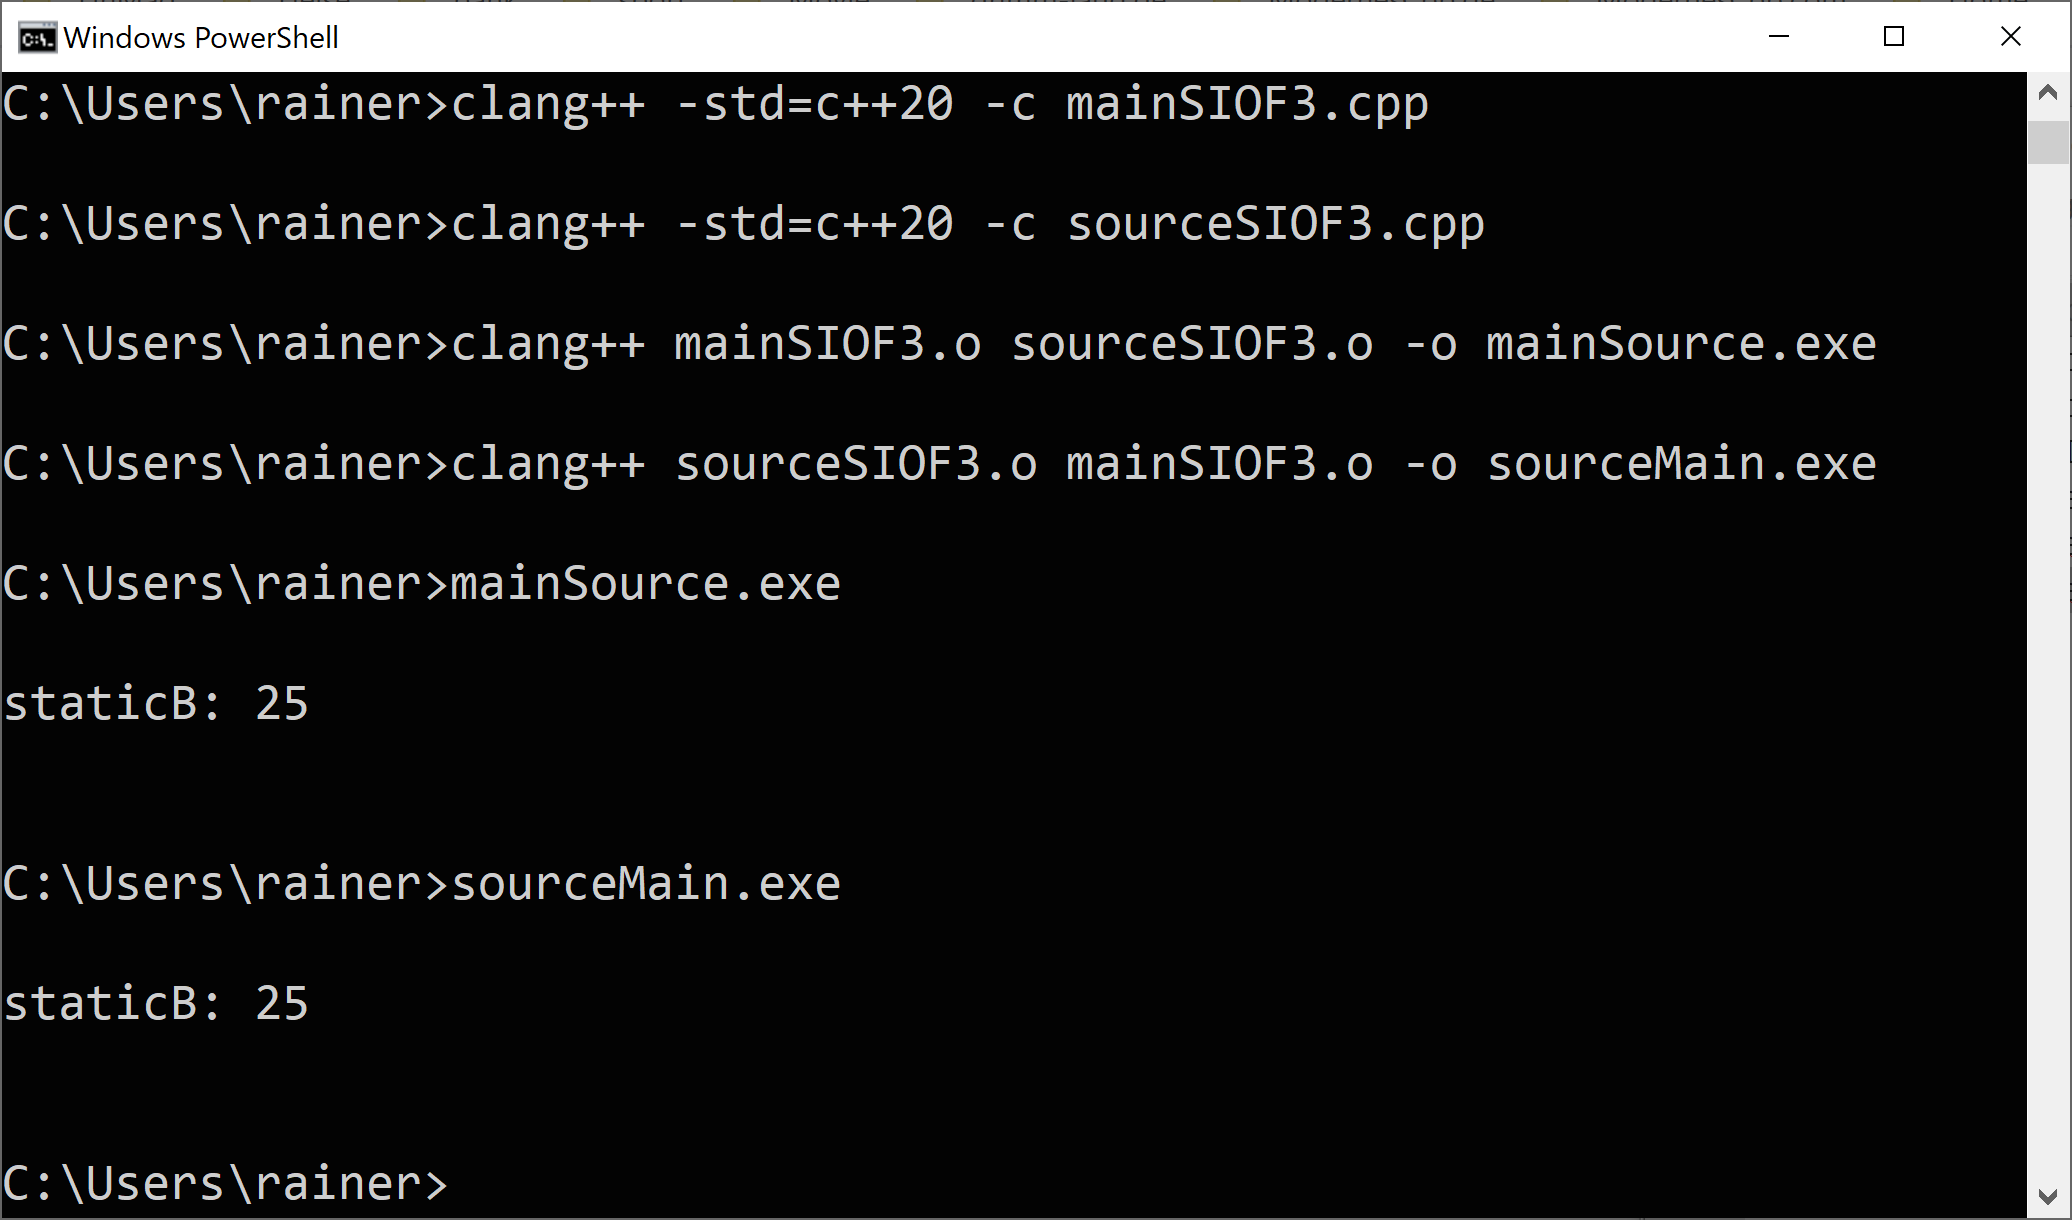
\includegraphics[width=0.6\textwidth]{content/3/chapter4/images/39.png}\\
用constinit解决静态初始化顺序错误
\end{center}

与使用本地静态变量进行延迟初始化一样,staticB的值为25。

\begin{tcolorbox}[breakable,enhanced jigsaw,colback=mygreen!5!white,colframe=mygreen!75!black,title={总结}]
\begin{itemize}
\item 
C++20中,新增了两个新的关键字:consteval和constinit。consteval生成一个在编译时执行的函数,constinit保证变量在编译时初始化。

\item 
与C++11中的constexpr相比,consteval保证函数在编译时执行。

\item 
const、constexpr和constinit之间是有区别的。const和constexpr创建常量变量。constexpr和constinit在编译时执行。
\end{itemize}
\end{tcolorbox}	

\newpage





